\documentclass[12pt,a4paper]{article}
\usepackage[slovene]{babel}
\usepackage[T1]{fontenc}
\usepackage{amsthm,amsfonts,amsmath,amssymb,url}
\usepackage{mathtools}
\usepackage{bm}
\usepackage{esvect}
\usepackage{bbm}
\usepackage{framed}
\usepackage{graphicx}
\usepackage{floatrow}
\usepackage{array}
\usepackage{multicol}
\usepackage{subcaption}
\usepackage[hidelinks]{hyperref}
\usepackage{listings}
\usepackage[margin=1in]{geometry}
\newcolumntype{L}{>{\centering\arraybackslash}m{3cm}}
\usepackage[svgnames]{xcolor}
\usepackage{minted}


\author{Gregor Vavdi, Nace Vreček}
\title{Računsko zahtevne metode \\
\large{Seminarska naloga\\
Manjkajoče vrednosti}}

\begin{document}
	\maketitle
	\pagebreak
	\tableofcontents


\newpage
\section{Cilj naloge}
Primerjanje uspešnosti razvrščanja v skupine z linearno diskriminantno analizo ob uporabi različnih metod za imputacijo manjkajočih vrednostih ter različnih mehanizmih manjkajočih vrednosti.


\section{Mehanizmi manjkajočih vrednosti in generiranje podatkov}

\subsection{MCAR}
\textit{Mehanizem povsem naključno manjkajočih podatkov. Verjetnost, da določena vrednost manjka je popolnoma neodvisna od manjkajočih vrednosti ter vrednosti pri ostalih spremenljivkah.}
\\

\noindent MCAR - Missing completly at random. Verjetnost, da določena vrednost manjka je popolnoma neodvisna od vrednosti ki manjka, kot od ostalih vrednosti (pri ostalih spremenljivkah). Delež manjkajočih vrednosti je bil enak pri vsaki spremenljivki. Za spremenljivke $X_2$, $X_3$ in $X_4$ sva generirala naključne števila z enakimi verjetnostmi na celotnem intervalu za vsako spremenljivko posebej.



\subsection{MAR}
\textit{Mehanizem naključno manjkajočih podatkov. Verjetnost, da vrednost manjka je neodvisna od manjkajoče vrednosti pogojno na vrednosti pri drugih spremenljivkah.}
\\

\noindent Pri mehanizmu MAR - missing at random sva se odločila za naslednje pogojene manjkajoče vrednosti. Spremenjivka $X_1$ vpliva na manjkajoče vrednosti $X_2, X_3$ in $X_4$.
\\
\noindent Povezanost med vrednostmi $X_1$ in manjkajočimi vrednostmi $X_2$ ($X_3$ in $X_4$) sva imenovala \textbf{moč} mehanizma. Ob večji povezanosti, dobimo večjo moč mehanizma. Moč sva definirala s črko $m$, kjer sva računala verjetnosti manjkajoče vrednosti za spremenljivko $X_1$:

$$p = \big| \frac{(X_1)^m}{(\sum_{i=1}^{n}X_1)^m} \big| $$


\noindent Izbirala sva med 5 različnimi vrednostmi $m: \{1, 2, 5, 8, 12  \}$. Spodaj so narisani grafi za lažjo predstavo. Narisani so na vzorcu N = 300 in 50\% manjkajočih vrednosti, za moč: $m = 1$  in $m= 12$, pri spremenljivki $X_3$:

\begin{figure}[ht]
	\centering
	\begin{minipage}[b]{.5\linewidth}	
		\centering
		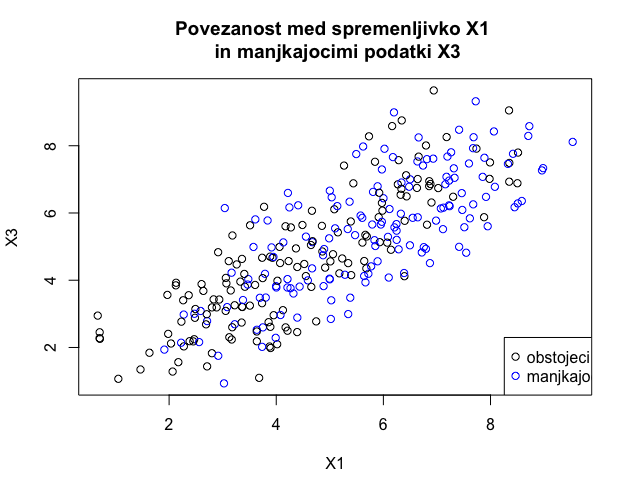
\includegraphics[width= 6cm, height = 6cm]{img/MAR_moc_1.png}
		\subcaption{Majhna moč (m = 1)}
		\label{fig:1a}
	\end{minipage}%
	\begin{minipage}[b]{.5\linewidth}
		\centering
		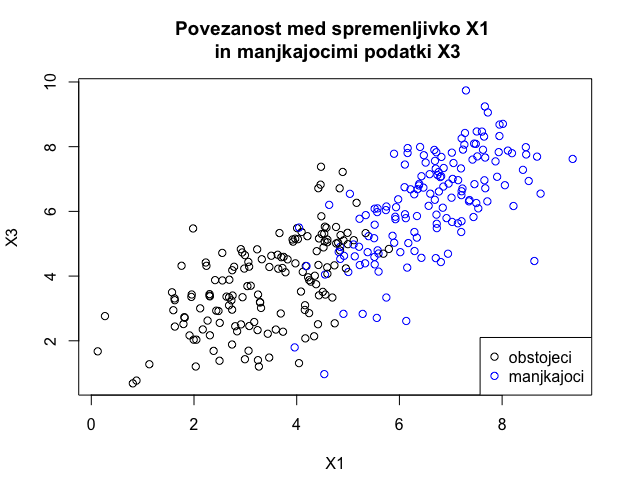
\includegraphics[width= 6cm, height = 6cm]{img/MAR_moc_12.png}
		\subcaption{Velika moč (m = 12) }
		\label{fig:1b}
	\end{minipage}
	\caption{Povezanost manjkajočih enot z obstoječimi pri $X_1$ in $X_3$}
	\label{fig:1}
\end{figure}

\begin{table}[ht]
	\centering
	\begin{tabular}{cccc}
		Delež NA & Skupina I & Skupina II  &  Skupina III  \\
		\hline
     0.3 & 19.55 & 30.53 & 39.92\\
     0.4 & 27.07 & 40.90 & 52.03\\
     0.5 & 34.97 & 51.32 & 63.71\\
     0.6 & 43.57 & 61.90 & 74.53\\
	\end{tabular}
	\caption{Delež NA vrednosti (v \%) v posamezni skupini, glede na celotni vzorec pri moči mehanizma m = 1}
	\label{tab:1}
\end{table}

	
\begin{table}[ht]
	\begin{tabular}{cccc}
		Delež NA & Skupina I & Skupina II  &  Skupina III  \\
		\hline
    0.3 & 0.46 & 15.18 & 74.37\\
    0.4 & 1.35 & 29.65 & 89.00\\
    0.5 & 3.93 & 49.60 & 96.47\\
    0.6 & 10.13 & 70.69 & 99.18\\
	\end{tabular}
	\caption{Delež NA vrednosti (v \%) v posamezni skupini, glede na celotni vzorec pri moči mehanizma m = 12}
	\label{tab:2}
\end{table}

\subsection{NMAR}

\textit{Mehanizem nenaključno manjkajočih podatkov. Verjetnost, da vrednost manjka je odvisna od manjkajoče vrednosti (torej od spremenljivke, ki ima manjkajočo vrednost).}
\\

\noindent Pri mehanizmu NMAR - \textit{Not missing at random} je spremenljivka direktno povezana s manjkajočimi vrednostmi. Tako sva manjkajoče vrednosti definirala na spremenljivki $X_2, X_3$ in $X_4$.
\\
\noindent Povezanost med vrednostmi $X_2$ ($X_3$ in $X_4$) in manjkajočimi vrednostmi $X_2$ ($X_3$ in $X_4$) sva, podobno kot prej,imenovala  \textbf{moč} mehanizma. Ob večji povezanosti, dobimo večjo moč mehanizma. Moč sva definirala s črko $m$, kjer sva računala verjetnosti manjkajoče vrednosti na isti spremenljivki.

$$p_i = \big| \frac{(X_i)^m}{(\sum_{i=1}^{n}X_i)^m} \big| $$

\noindent za $i = 1,2,3$.
\newpage
\noindent Izbirala sva med 5 različnimi vrednostmi $m: \{1, 2, 5, 8, 12  \}$. Spodaj so narisani grafi za lažjo predstavo. Narisane so na vzorci N = 300 in 50\% manjkajočih vrednosti, za moč: $m = 1$  in $m= 12$, pri spremenljivkah $X_3$:


\begin{figure}[ht]
	\centering
	\begin{minipage}[b]{.5\linewidth}	
		\centering
		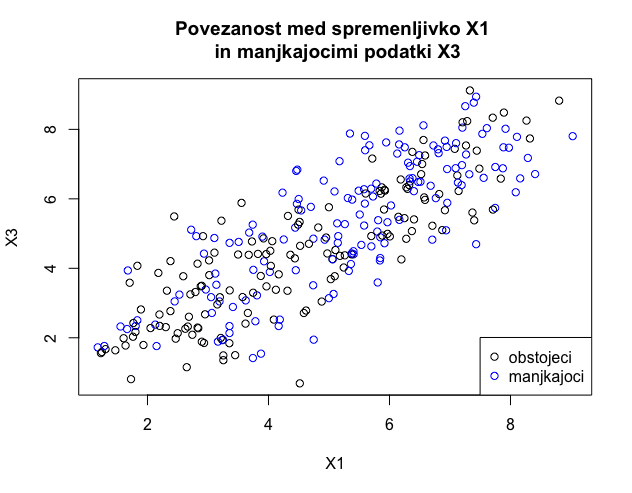
\includegraphics[width= 7cm, height = 7cm]{img/NMAR_moc_1.png}
		\subcaption{Majhna moč (m = 1)}
		\label{fig:2a}
	\end{minipage}%
	\begin{minipage}[b]{.5\linewidth}
		\centering
		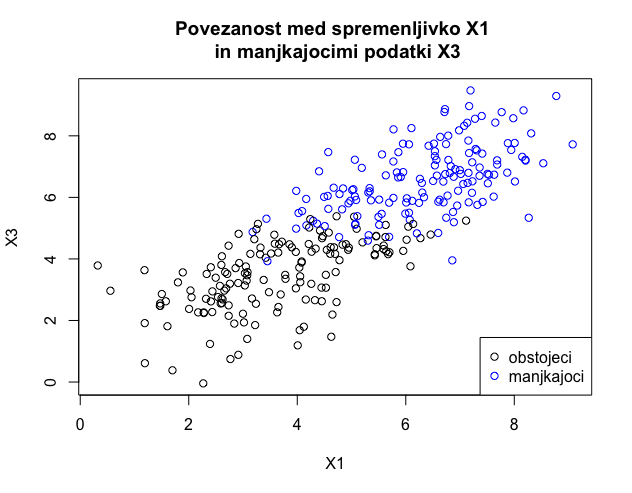
\includegraphics[width= 7cm, height = 7cm]{img/NMAR_moc_12.png}
		\subcaption{Velika moč (m = 12) }
		\label{fig:2b}
	\end{minipage}
	\caption{Povezanost manjkajočih enot z obstoječimi pri $X_1$ in $X_3$}
	\label{fig:2}
\end{figure}


\begin{table}[ht]
	\centering
	\begin{tabular}{cccc}
		Delež NA & Skupina I & Skupina II  &  Skupina III  \\
		\hline
      0.3 & 19.57 & 30.47 & 39.95\\
      0.4 & 26.76 & 40.90 & 52.34\\
      0.5 & 34.80 & 51.39 & 63.81\\
      0.6 & 43.58 & 62.06 & 74.36\\
	\end{tabular}
	\caption{Delež NA vrednosti (v \%) v posamezni skupini, glede na celotni vzorec pri moči mehanizma m = 1}
	\label{tab:3}
\end{table}

	
\begin{table}[ht]
	\begin{tabular}{cccc}
		Delež NA & Skupina I & Skupina II  &  Skupina III  \\
		\hline
    0.3 & 0.48 & 15.08 & 74.44\\
    0.4 & 1.36 & 29.62 & 89.02\\
    0.5 & 3.93 & 49.59 & 96.48\\
    0.6 & 10.07 & 70.74 & 99.19\\
	\end{tabular}
	\caption{Delež NA vrednosti (v \%) v posamezni skupini, glede na celotni vzorec pri moči mehanizma m = 12}
	\label{tab:4}
\end{table}


\pagebreak

\section{Metode imputacij}

\subsection{Analiza na podlagi popolnih enot}
Analiza na podlagi popolnih enot (listwise deletion) je smiselna kadar velja MCAR mehanizem in je delež manjkajočih vrednosti majhen. V literaturi lahko zasledimo, da je taka metoda primerna v primerih, ko je delež manjkajočih vrednosti manjši od 5 \% (Graham, 2009). Predpostavka o MCAR mehanizmu je močna in v praksi pogosto kršena, kar lahko privede do pristranskih ocen in manjši moči (Graham, 2009).



\subsection{Multiple imputacije preko verižnih enačb (MICE)}
Metoda MICE prihaja iz družine multiplih imputacij. Torej generiramo več ločenih podatkovij z imputiranimi vrednostmi (metodo imputiranja manjkajočih vrednosti določimo sami). Funkcija \emph{mice} iz istoimenskega paketa kot metodo imputiranja uporablja \emph{predictive mean matching}. Za vsako manjkajočo vrednost prediktorja izberemo majhen set kandidatov (cca. 10), ki nimajo manjkajočih vrednosti ter imajo napovedane vrednosti najbližje napovedani vrednosti manjkajočega prediktorja. Izmed tega seta kandidatov naključno izberemo eno vrednost ter s to vrednostjo nadomestimo manjkajočo vrednost prediktorja. Glavna predpostavka MICE metode je, da mora biti porazdelitev manjkajočih vrednosti enaka porazdelitvi opazovanih vrednosti ter, da je mehanizem manjkajočih vrednosti MCAR.\\
Kot optimalno število imputiranih podatkovij literatura navaja vrednosti od 5-10 (White et al., 2010). Za potrebe najine seminarske naloge sva izbrala 10 imputiranih podatkovij ter 5 iteracij za vsako podatkovje.

\subsubsection{Koraki:}
\begin{enumerate}
    \item 
    Vrednosti imputiramo z enostavno metodo (v najinem primeru je to \emph{predictive mean matching})
    \item
    Ocenimo model za eno (vsako spremenljivko, ki ima manjkajoče vrednosti) spremenljivko, na podlagi imputiranega podatkovja iz 1. koraka.
    \item
    Na podlagi modela iz točke 2. imputiramo nove vrednosti za manjkajoče vrednosti
    \item
    Ponavljamo koraka 2 in 3 (za vse spremenljivke z manjkajočimi vrednostmi) dokler se porazdelitve parametrov v točki 2 ne stabilizirajo (imputacije iz 3. točke predstavljajo eno imputirano podatkovje)
    \item
    Ponavljamo korake 1-4, da dobimo željeno število imputiranih podatkovij oziroma dosežemo konvergenco imputiranih vrednosti
\end{enumerate}

\subsection{Imputacije preko slučajnih gozdov}
Metoda imputacij preko slučajnih gozdov je primerna tako za kvalitativne kot za kvantitavitne spremenljivke. Metoda deluje po principu napovedovanja manjkajočih vrednosti preko slučajnih gozdov, ki so bili izdelani za vsako spremenljivko (prediktor), ki ima manjkajoče vrednosti, na ne-manjkajocih vrednostih ter ta postopek ponavljamo, s tem, da vsako iteracijo posodobimo manjkajoče vrednosti z napovedmi modela, dokler ne dosežemo željene natančnosti (razlike med i in $i_{-1}$ iteracijo) (Stekhoven \& Bühlmann, 2011).

\subsubsection{Psevdo algoritem:}
\begin{verbatim}
    1. Matrika X, velikosti nxp, zaključitveni kriterij Gama
    2. Vrednosti imputiramo z enostavno metodo
    3. Vektor k v katerem so spremenljivke urejene glede na delež 
    manjkajočih vrednosti (naraščajoč vrstni red)
    
    while not Gama do:
        X_old_imp  ; shranimo imputirano matriko
        for s in k:
            random forest y_obs_s x_obs_s
            napovemo y_miss_s
            z napovedmi y_miss_s posodobimo matriko X_old_imp
        end for
    end while
    return X_old_imp
\end{verbatim}



\subsection{Metoda imputacij na podlagi najbližjih sosedov (kNN)}
Metoda imputacij na podlagi najbližjih sosedov je metoda, ki temelji na podobnosti (oz. razdalji) med podatki (Beretta \& Santaniello, 2016). Algoritem za ocenjevanje manjkajočih vrednosti uporabi samo popolne enote. Za oceno manjkajoče vrednosti na spremenljivki $x1$, pogledamo $k$ vrednosti enot spremenljivke $x1$, katerih vrednosti so najbolj podobne vrednosti enote, ki ima manjkajočo vrednost. Glede optimalne določitve $k$ ni jasnega konsenza. Tako sta Lall in Sharma (1996), kot primerno metodo ocenjevanja optimalnega števila najbližjih sosedov podala enačbo $k = \sqrt{n}$, če je $n > 100$. Kot metodo imputiranja manjkajočih vrednosti sva izbrala metodo obteženih povprečij. Uteži se izračunajo kot $e^{-d(k,x)}$, kjer $d$ predstavlja Evklidsko razdaljo med enoto z manjkajočo vrednostjo ($x$) ter $k-tim$ sosedom.\\
Predpostavka kNN metode je, da lahko napovemo manjkajočo vrednost, na podlagi podobnih vrednosti drugih spremenljivk, ki nimajo manjkajočih vrednosti, torej, da obstaja povezanost med spremenljivko z manjkajočo enoto ter ostalimi spremeljivkami.\\
Za potrebe seminarske naloge sva nastavila $k$ (število najbližjih sosedov) na 10.\\

\subsection{EM algoritem}

EM-algortem temelji na dveh predpostavkah. Opazovane vrednosti so neodvisne v p razsežnem normalnem prostoru s parametri $\mu$ in $\Sigma$. Algoritem ocenjuje po metodi največjega verjetja. Druga predpostavka pravi, da podatki manjkajo naključno (MCAR) in neodvisno, vendar tako, da nikoli ne manjkajo vse komponente.

V praksi sva uporabila programsko knjižnico \verb|norm| in njene funkcije \verb|em.norm|, ki naredi EM - algoritem na nepopolnih podatkih za vsako skupino posebaj. Potem sva z funkcijo \verb|getparam.nor|, kjer sva dobila parametre porazdelitve za vsako skupino posebaj. Te parametre sva uporabila za generiranje novih podatkov, za vsako skupino posebaj. Potem sva združila nepopolni set in zamenjala NA vrednosti z novimi generiranimi podatki, za vsako skupino posebej. Nato sva združila v eno podatkovje in izvedla LDA.

\pagebreak

\section{Simulacija}

Simulacijo sva razdelila na tri dele glede na tri mehanizme manjkajočih vrednosti. V vsakem delu preko razvrščanja v skupine z LDA preverjala uspešnost imputacijskih metod (za referenco sva uporabila uspešnost razvrstitve LDA modela na popolnem podatkovju).\\
Originalno (popolno) podatkovje sva generirala iz multivariatne normalne porazdelitve ter glede na mehanizem manjkajočih vrednosti (MAR, MCAR, NMAR) uvedla manjkajoče vrednosti (katerih delež se je spreminjal tekom simulacije). Kot končno mero uspešnosti sva uporabila delež pravilno razvrščenih enot na novem podatkovju, brez manjkajočih vrednosti.

\subsection{Fiksni dejavniki}
\begin{itemize}
    \item Število spremenljivk; 4
    \item Število skupin; 3
    \item Velikost skupin; 100, 100, 100
    \item Povprečja skupin; 3, 5, 7
    \item Varianca spremenljivk; 1
    \item Korelacija med spremenljivkami; 0.3
    \item Porazdelitev spremenljivk; multivariatna normalna
    \item Število spremenljivk z manjkajočimi vrednostmi; 3
\end{itemize}   


\subsection{Variabilni dejavniki}
\begin{itemize}
    \item Mehanizem manjkajočih vrednosti; MCAR, MAR, NMAR
    \item Moč mehanizma manjkajočih vrednosti (pri MAR in NMAR); 1, 2, 5, 8, 12
    \item Metoda imputacije manjkajočih vrednosti
    \item Delež manjkajočih vrednosti; 0.3, 0.4, 0.5, 0.6
\end{itemize}

\pagebreak

\section{Rezultati}

\subsection{Rezultati MCAR}

\begin{figure}[ht]
	\centering
	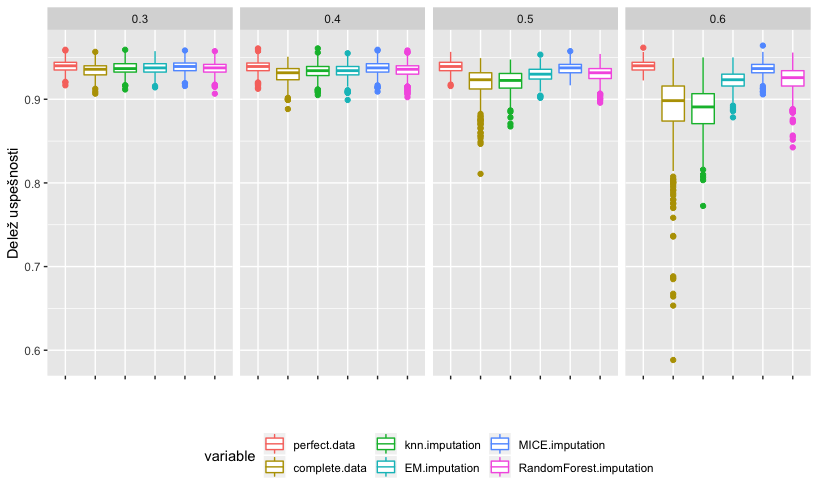
\includegraphics[width= 12cm, height = 7cm]{img/MCAR_boxplot.png}
	\caption{Variabilnost deleža pravilno razvrščenih enot pri mehanizmu MCAR} 
	\label{fig:3}
\end{figure}

\noindent Na sliki 3 lahko vidimo, da variabilnost ocen z naraščanjem deleža manjkajočih vrednosti postopoma narašča, predvsem pa je očiten porast pri metodi popolnih enot, ko variabilnost narašča hitreje kot pri ostalih metodah.

%Variabilnost je povsod približno enaka (0.01), razen pri complete cases, kjer pri velikem deležu NA vrednosti, naraste do 0.04. Govoriva od SD.



\begin{figure}[ht]
	\centering
	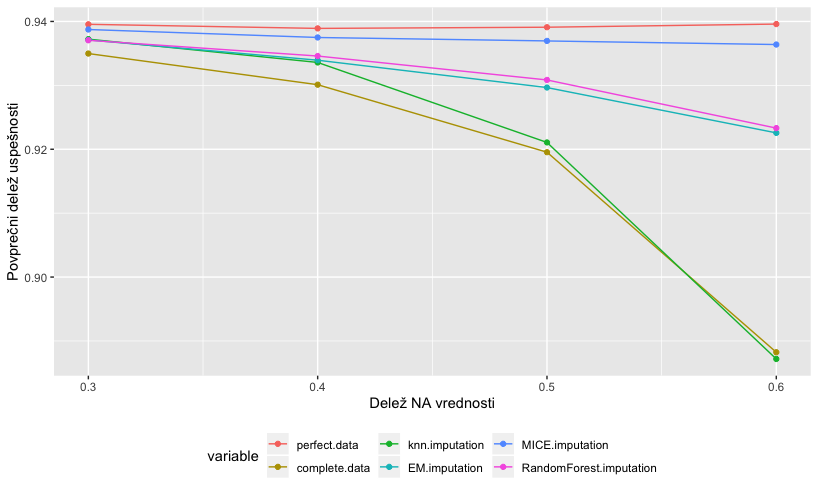
\includegraphics[width= 12cm, height = 7cm]{img/MCAR_mean_line.png}
	\caption{Povprečje uspešnosti pri mehanizmu MCAR za različne deleže manjkajočih vrednosti} 
	\label{fig:4}
\end{figure}

\noindent Kot prikazuje slika 4, uspešnost razvrstitve pada z naraščanjem deleža manjkajočih vrednosti, vendar se hitrost padanja razlikuje med metodami. Najslabše razvrstitve je vrnila metoda z EM algoritmom, kNN metoda in metoda popolnih enot sta si precej podobni, razen v začetni razvrstitvi, ko je delež manjkajočih enot enak 0.3. Najboljše rezultate je vrnila metoda MICE, za katero lahko vidimo, da ima rezulate precej podobne razvrstitvi na celotnem podatkovju, prav tako pa uspešnost z višanjem deleža manjkajočih vrednosti ne pada tako hitro kot pri ostalih metodah.

\pagebreak

\subsection{Rezultati MAR}

\begin{figure}[ht]
	\centering
	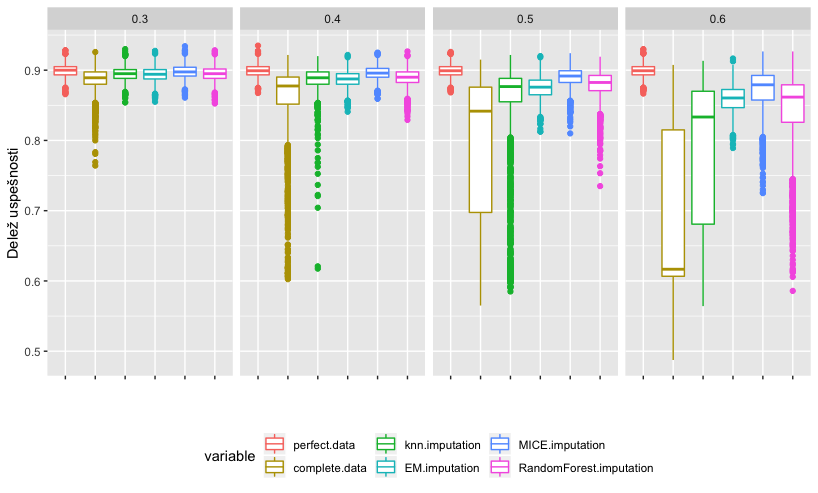
\includegraphics[width= 12cm, height = 7cm]{img/MAR_boxplot.png}
	\caption{Variabilnost deleža pravilno razvrščenih enot pri mehanizmu MAR} 
	\label{fig:5}
\end{figure}

\noindent Variabilnost na sliki 5 je podana samo glede na delež manjkajočih vrrednosti, ne pa tudi upoštevajoč moč mehanizma, kajti variabilnost metod se ni bistveno razlikovala med različnimi močmi mehanizma MAR. Pri nizkem deležu manjkajočih enot vidimo, da je variabilnost uspešnosti razvrstitve met metodami primerljiva. Z naraščanjem deleža manjkajočih enot se variabilnost povečuje pri vseh metodah, največja razlika v variabilnosti pa je pri metodah na popolnih enotah ter kNN metodi. Najmanjša razlika v variabilnosti uspešnosti razvrstitve, glede na delež manjkajočih vrednosti je pri metodi MICE, sledi pa ji EM algoritem.
 

%Variabilnosti nisem dal kot tabelo, ker je preveč različnih. Lahko rečeš, da je največja variabilnost (sd) pri complete.data (od 0.02 do 0.12) in knnImputation (od 0.01 do 0.10). Vsi ostali imajo variabilnost bistveno manjšo (od 0.05 do 0.02) ne upoštevajoč dejavnik moči mehanizma

\begin{figure}[ht]
	\centering
	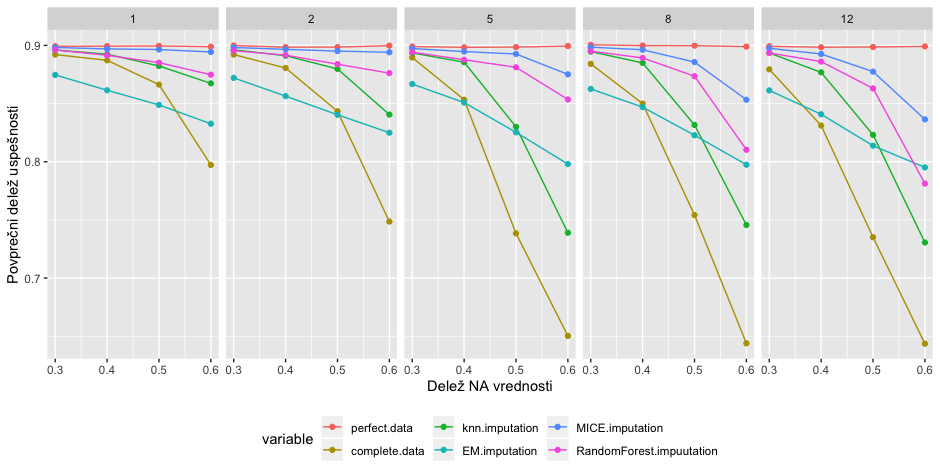
\includegraphics[width= 12cm, height = 7cm]{img/MAR_line_mean.png}
	\caption{Povprečje uspešnosti pri mehanizmu MAR za različne deleže manjkajočih vrednosti in moči mehanizma} 
	\label{fig:6}
\end{figure}

\noindent Slika 6 prikazuje povprečno uspešnost razvrstitve enot glede na delež manjkajočih vrednosti ter moč mehanizma MAR. Opazimo, da je uspešnost razvrstitve pri metodi MICE pri nizki moči (1 in 2) primerljiva z razvrstitvijo na originalnem podatkovju (brez manjkajočih vrednosti), z večanjem moči pa metoda MICE dosega vedno slabše rezultate. Pri nizki moči sta metodi kNN in metoda slučajnih gozdov primerljivi, z večanjem moči ter deležem manjkajočih vrednosti pa uspešnost razvrstitve pada hitreje pri metodi kNN kot pri metodi slučajnih gozdov. Izmed imputacijskih metod je, pri nizki moči ter nizkih deležih manjkajočih vrednosti, EM algoritem dosegel najslabše rezulate, z višanjem moči mehanizma manjkajočih vrednosti ter deležem manjkajočih vrednosti pa slabše rezultate vrneta metodi kNN in metoda slučajnih gozdov. Pričakovano uspešnost razvrstitve z metodo narejeno na  popolnih podatkih, pada najhitreje. 


\subsection{Rezultati NMAR}

\begin{figure}[ht]
	\centering
	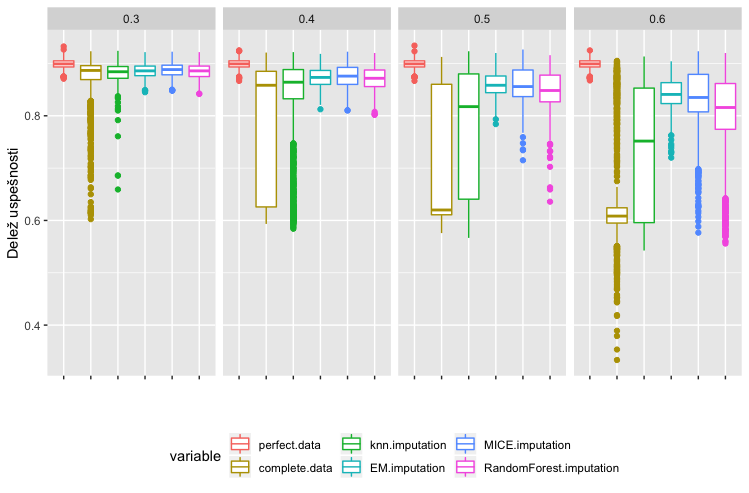
\includegraphics[width= 12cm, height = 7cm]{img/NMAR_boxplot.png}
	\caption{Variabilnost deleža pravilno razvrščenih enot pri mehanizmu NMAR} 
	\label{fig:7}
\end{figure}

\noindent Variabilnost na sliki 7 je podana samo glede na delež manjkajočih vrrednosti, ne pa tudi upoštevajoč moč mehanizma, kajti variabilnost metod se ni bistveno razlikovala med različnimi močmi mehanizma NMAR. Pri nizkem deležu manjkajočih enot je variabilnost uspešnosti razvrščanja med metodami primerljiva, odstopata metodi EM algoritem in metoda popolnih enot. Z večanjem deleža manjkajočih vrednosti se variabilnost povečuje pri vseh metodah, najbolj pa je to očitno pri metodi kNN ter metodi popolnih enot.

\pagebreak

\begin{figure}[ht]
	\centering
	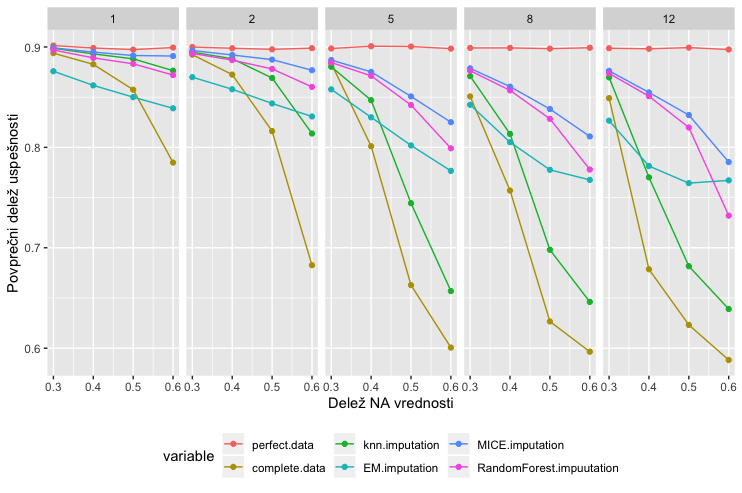
\includegraphics[width= 12cm, height = 7cm]{img/NMAR_mean_line.png}
	\caption{Povprečje uspešnosti pri mehanizmu NMAR za različne deleže manjkajočih vrednosti in moči} 
	\label{fig:8}
\end{figure}

\noindent Slika 8 prikazuje povprečno uspešnost razvrstitve enot glede na delež manjkajočih vrednosti ter moč mehanizma NMAR. Pri moči mehanizma 1 je uspešnost razvrstitve pri metodi MICE podobna razvrstitvi na originalnem podatkovju (brez manjkajočih vrednosti). Z večanjem moči mehanizma manjkajočih vrednosti se uspešnost razvrstitve slabša pri vseh metodah, poleg metode popolnih enot pa najslabše rezultate dosega metoda kNN. Izmed vseh uporabljenih metod je metoda MICE dosegla najboljše rezultate.  


\pagebreak
\section{Zaključek}

Cilj seminarske naloge je bil preverjanje uspešnosti različnih metod imputacije, preko razvrščanja v skupine z linearno diskriminantno analizo. Večina imputacijskih metod predpostavlja MCAR oziroma MAR mehanizem manjkajočih vrednosti, zato sva poelg tega vključila tudi NMAR mehanizem ter preverjala vpliv moči mehanizma (verjetnosti za manjkajočo vrednost) ter delež manjkajočih vrednosti. Pri vseh mehanizmih manjkajočih vrednosti je najboljše razvrstitve vrnil LDA model, narejen na imputiranem podatkovju z metodo MICE. Pri MAR mehanizmu so bile razvrstitve pri metodi MICE malo nižje kot razvrstitev narejena na originalnem podatkovju (brez manjkajočih vrednosti). Pri MAR in NMAR mehanizmu je uspešnost razvrstitve padala z večanjem moči mehanizma, vendar je bila še vedno višja kot pri ostalih metodah. Variabilnost uspešnosti razvrstitve je bila v primeri MCAR in MAR najnižja pri metodi MICE, pri NMAR pa je bila najnižja variabilnost pri EM algoritmu.\\
Izmed izbranih imputacijskih metod priporočava metodo MICE, vendar pa je pri interpretaciji rezultatov potrebna previdnost, saj v večini primerov ne poznamo mehanizma manjkajočih vrednosti. Prav tako sva v najini seminarski nalogi preverjala imuptacijske metode zgolj za številske spremenljivke.

    
 

\newpage
\begin{thebibliography}{9}
\bibitem{kNN}
Beretta, L., Santaniello, A. (2016).
\textit{Nearest neighbor imputation algorithms: a critical evaluation.}
BMC Med Inform Decis Mak. 2016;16(Suppl 3):74. doi: 10.1186/s12911-016-0318-z.
\bibitem{EM}
Geoffrey J. M., \& Thriyambakam K. (1997) 
\textit{The EM Algorithm and Extensions.} 
Wiley Series in Probability and Statistics
\bibitem{Listwise} 
Graham, J. W. (2009). 
\textit{Missing data analysis: Making it work in the real world.} 
Annual Review of Psychology, 60(1), 549–576. doi:10.1146/annurev.psych.58.110405.085530 
\bibitem{NNboot}
Lall, U. \& Sharma, A. (1996).
\textit{A nearest-neighbor bootstrap for resampling hydrologic time series.}
Water Resources Research 32 (3), 679–693.
\bibitem{missForest}
Stekhoven, D. J., \& Bühlmann, P. (2011).
\textit{MissForest: non-parametric missing value imputation for mixed-type data.}
Bioinformatics, 28(1):112-118.
\bibitem{MICE}
White, I. R., Royston, P., Wood, M. A. (2010)
\textit{Multiple imputation using chained equations: Issues and guidance for practice.}
Stat Med, 30 (2011), pp. 377-399

\end{thebibliography}

\end{document}